\documentclass[a4paper, 12pt]{article}
\usepackage[utf8]{inputenc}
\usepackage[brazil]{babel}
\usepackage{amstext} 	% need for \text command
\usepackage{amsmath}    % need for subequations
\usepackage{graphicx}   % need for figures
\usepackage{verbatim}   % useful for program listings
\usepackage{color}      % use if color is used in text
\usepackage{subfigure}  % use for side-by-side figures
\usepackage{hyperref}   % use for hypertext links, including those to external documents and URLs
\usepackage{pictexwd}	% use for pictex graphs

%\author{Vítor M. Martins}
\title{PME2360}

\begin{document}
\maketitle
%\newpage
%\tableofcontents
%\newpage

\section*{8}

\begin{enumerate}
\item 8.1 considerações fluido dinamicas
\item 8.2 consideraçoes termicas
\item 8.3 balanco de energia
\item 8.4 escoamento laminar em tubos circulares
\begin{itemize}
\item regime plenamente desenvolvido
\item regiao de entrada
\end{itemize}
\item 8.5 escoamento turbulento em tubos circulares
\item 8.6 tubos nao circulares
\end{enumerate}

\subsection*{8.1 Consideracoes fluido-dinamicas}
\begin{figure}[h]
\begin{center}
\includegraphics[scale=0.68]{./fig/1a.png}
\caption{\label{fig:1}Desenlvolvimento da C. L. fluidodinâmica laminar num tubo circular} 
\end{center}
\end{figure}

\[R_{eD}= \frac{\rho \bar{u} D }{\mu } = \frac{\bar{u} D}{\upsilon}\]

\[R_{eD,critico}=2300\]
Escoamento laminar:
\[\frac{X_{CD,\upsilon}}{D} = 0.05R_{eD}\] 
Escoamento turbulento:
\[\frac{X_{CD,\upsilon}}{D} = 10\] 

No escoamento laminar:

\[u_{m}= - \frac{r_{0}^{2}}{8\mu} \frac{dp}{dx}\]
\[f = \frac{-\frac{dp}{dx}}{\frac{1}{2}\rho u_{m}^{2}}\]

\[c_{f}=\frac{\tau_{\Delta}}{\frac{1}{2}\rho u_{m}^{2}}\]

Demonstra-se que: 
\[c_{f} = \frac{f}{4}\]
Escoamento laminar: 
\[f= \frac{64}{Re_{d}}\]

Escoamento turbulento (tubo liso): 
\[f=0.316 Re_{D}^{-\frac{1}{4}}\]
\[Re_{D} <= 2 * 10^{4}\]

\[f=0.316 Re_{D}^{-\frac{1}{4}}\]
\[Re_{D} >= 2*10^{4}\]

\[ f = (0.790 \ln (Re_{D} -1.64))^{-2}\ \ \ \ \ \ \ 3000 <= Re_{D} <= 5 * 10^{6} \]

\subsection*{8.2 Considerações térmicas}

\begin{figure}[h]
\begin{center}
\includegraphics[scale=0.21]{./fig/2a.png}
\caption{\label{fig:2}Desenvolvimento da C. L. térmica laminar num tubo circular} 
\end{center}
\end{figure}

escoamento laminar: 
\[\frac{Xc_{D,t}}{D}=0.05Re_{D}Pr\]
escoamento turbulento:
\[\frac{Xx_{D,t}}{D}=10\]

\[q''_{s}=h(T_{S}-T_{m})\]

\subsection*{8.3 Balanço de Energia}

\begin{enumerate}
\item reg. permanente
\item liq. incompressivel
\item dissipacao viscosa e desprezivel
\item trans. calor por condução na direção x desprezível
\item propriedades constantes
\end{enumerate}


tubo:

\[m_{c} ( T_{M}|_{x} - ( T_{M}|_{x} + \frac{dT_{m dx}}{dx} ) ) + dq_{conv} = 0\]

\[\frac{dT_{m dx}}{dx} = - \frac{dq_{conv}}{\dot{m}c}\]

\[\frac{dT_{M} dx}{dx} = \frac{q''_{s} Pdx}{\dot{m}c}\]

\[\frac{dT_{M}}{dx}= \frac{q''_{S} P}{\dot{m}c} = \frac{h(T_{S} - T_{m}) P}{\dot{m}c}\]

fluxo de calor uniforme na superficie:

\[\frac{dT_{m}}{dx}= \frac{q''_{S}}{\dot{m}c}\]

Condições iniciais: x=0, Tm = $T_{m,e}$

\[T_{m}= \frac{q''_{s}Px}{\dot{m}c}+T_{m,e}\]

\begin{figure}[h]
\begin{center}
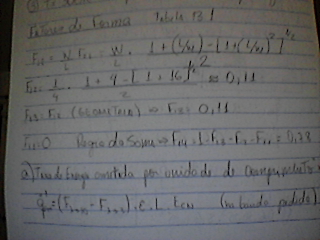
\includegraphics[scale=0.48]{./fig/3.png}
\caption{\label{fig:tur}Grafico T x X } 
\end{center}
\end{figure}

Temperatura superficial uniforme:
\[ \frac{dT_{m}}{dx} = \frac{hP(T_{S}-T_{m})}{\dot{m}c}\]

\[\theta=T_{S}-T_{m} \]

Logo $d \theta = -dT_{m}$

\[\frac{d\theta}{dx}=-\frac{hP}{\dot{m}c}\theta\]

\[\ln (\theta)|_{\theta_{e}}^{\theta}= - \frac{hPx}{\dot{m}c}\]

\[\frac{\theta}{\theta_{e}}= \exp (- \frac{hPx}{\dot{m}c})\]

\[\frac{T_{m}-T_{s}}{T_{m,e}-T_{s}}= \exp (- \frac{hPx}{\dot{m}c})\]

\subparagraph*{8.4 Escoamento laminar em tubos circulares}

\paragraph*{reg desenvolvida}

Para $q''_{S}\ cte$: 
\[N_{Ud}=4.36\]
Para $T_{S}\ cte$: 
\[N_{Ud}=3.66\]

\paragraph*{reg. de entrada}

$T_{S}\ cte$

\[\bar{N}_{UD}=3.66+\frac{0.668(D/L)Re_{D}P_{r}}{1+0.04[((D/L)Re_{D}Pr)]^{\frac{2}{3}}}\]

Onde $[((D/L)Re_{D}Pr)]$ é o numero de Graetz ($Gz_{D}$) e com 
\[\bar{N}_{UD}=\frac{\bar{hD}}{k} \]

Válida para comprimento de entrada e comprimento de entrada combinada se $Pr >=5$

\subparagraph*{Seidel e Tate (comp. de entrada comb.)}

\[\bar{N}_{UD}=1.86( \frac{Re_{D}Pr}{L/D} )( \frac{\mu}{\mu_{S}} )\]

com $N_{Ud}>3.66$

\[0.6 <= Pr <= 5\]

\[0.0044 <= \frac{\mu}{\mu_{S}} <= 9.75\]

\subsection*{8.5 Escoamento turbulento em tubos circulares}

Dittus-Boelter: 
\[N_{UD}=0.023Re_{D}^{\frac{4}{5}}(Pr)^{n}\]
Com n = 0.4, $Ts > Tm$ e $0.7 <=Pr<=100$
E para n = 0.3, $Ts < Tm$ e $Re_{D}>=10000, L/D >=10$

\paragraph*{Bibliografia} Figuras retiradas de Incropera - Fundamentals of Heat and Mass Transfer-Incropera (6a edicao)

\end{document}